% \settocdepth{chapter}
\chapter{计算双曲正切函数的傅立叶变换}
\label{appendices a}

\begin{equation}
    \begin{aligned}
      &  \int_{-\infty }^{\infty } \tanh (x)e^{-ikx}dx= \\
&=\int_{-\infty}^{\infty} \frac{e^{x}-e^{-x}}{e^{x}+e^{-x}} e^{-i kx} d x \\
&=\int_{-\infty }^{\infty } e^{-ikx}dx-\int_{-\infty }^{\infty } \frac{2e^{-ikx}}{e^{2x}+1} dx \\
\end{aligned}
\end{equation}

先计算积分第一项:
\begin{equation}\label{}
    \begin{aligned}
        &  \int_{-\infty}^{\infty} e^{-i k x} d x=\lim _{\alpha \rightarrow \infty}  \int_{-\alpha}^{\alpha} e^{-i k x} d x \\
        &=\left.\lim _{\alpha \rightarrow \infty}  \frac{-e^{-i k x}}{i k}\right|_{-\alpha} ^{\alpha} \\
         &= \lim _{\alpha \rightarrow \infty} \frac{1}{ik} (e^{i \alpha k}-e^{-i \alpha k})\\
        &=\lim _{\alpha \rightarrow \infty} \frac{2i}{ik} \sin \alpha k=2\pi\delta(k) .
        \end{aligned}
\end{equation}
下面证明$\lim _{\alpha \rightarrow \infty} \frac{\sin \alpha k}{\pi k} =\delta(k)$。首先证明它的积分等于1。注意到:
\begin{equation}\label{}
    \begin{aligned}
        &I=\int_{0}^{\infty} e^{-\gamma x} \cos \beta x d x=\left.e^{-\gamma x} \frac{\sin \beta x}{\beta}\right|_{0} ^{\infty}+\frac{\gamma}{\beta} \int_{0}^{\infty} e^{-\gamma x} \sin \beta x d x\\
        &=\frac{\gamma}{\beta} \int_{0}^{\infty} e^{-\gamma x} \sin \beta x d x=-\left.\frac{\gamma}{\beta^{2}} e^{-\gamma x} \cos \beta x\right|_{0} ^{\infty}-\frac{\gamma^{2}}{\beta^{2}} \int_{0}^{\infty} e^{-\gamma x} \cos \beta x d x \\
        &=\frac{\gamma}{\beta^{2}}-\frac{\gamma^{2}}{\beta^{2}} I
    \end{aligned}
\end{equation}
解得:
\begin{equation}\label{I1}
    I=\int_0^{\infty} e^{-\gamma x} \cos \beta x d x=\frac{\gamma}{\beta^2+\gamma^2}, \quad \gamma>0
    \end{equation}
将式\ref{I1}的等式两边对$\beta$从0到$\alpha$进行积分,得
\begin{equation}\label{}
    \begin{aligned}
        & \int_0^\alpha d \beta\left(\int_0^{\infty} e^{-\gamma x} \cos \beta x d x\right)=\int_0^{\infty} d x e^{-\gamma x}\left(\int_0^\alpha d \beta \cos \beta x\right) \\
        = & \int_0^{\infty} d x e^{-\gamma x} \frac{\sin \alpha x}{x}=\int_0^\alpha d \beta \frac{\gamma}{\beta^2+\gamma^2}=\arctan \frac{\alpha}{\gamma} .
        \end{aligned}
\end{equation}
于是有
\begin{equation}\label{}
    \lim _{\gamma \rightarrow 0} \int_0^{\infty} d x e^{-\gamma x} \frac{\sin \alpha x}{x}=\int_0^{\infty} d x \frac{\sin \alpha x}{x}=\lim _{\gamma \rightarrow 0} \arctan \frac{\alpha}{\gamma}=\arctan \infty=\frac{\pi}{2}
\end{equation}
再通过等式变化,就可以完成证明。
可以看出,第一项积分可以化为$\delta$函数,当$k>0$时为零;下面计算第二项积分,计算第二项积分需要使用留数定理,由于被积函数中的$\frac{1}{e^{2x}+1}$存在无穷多个奇点,为了避免计算无穷多个奇点,令$t = e^x$,在上半圆形,逆时针的围道上只需要计算一个奇点$t = i$的留数即可。下面是计算第二项积分的主要步骤:
\begin{equation}\label{2ji}
\begin{aligned}
    &  \int_{-\infty }^{\infty } \frac{e^{-ikx}}{e^{2x}+1} dx\\
    &\overset{令t=e^x}{=}\int_{0 }^{\infty } \frac{t^{-ik}}{t^2+1}\frac{dt}{t}.
\end{aligned}
\end{equation}
为了使用留数定理,给出一个逆时针半圆围道:
% \begin{figure}[htbp]
%     \centering
%     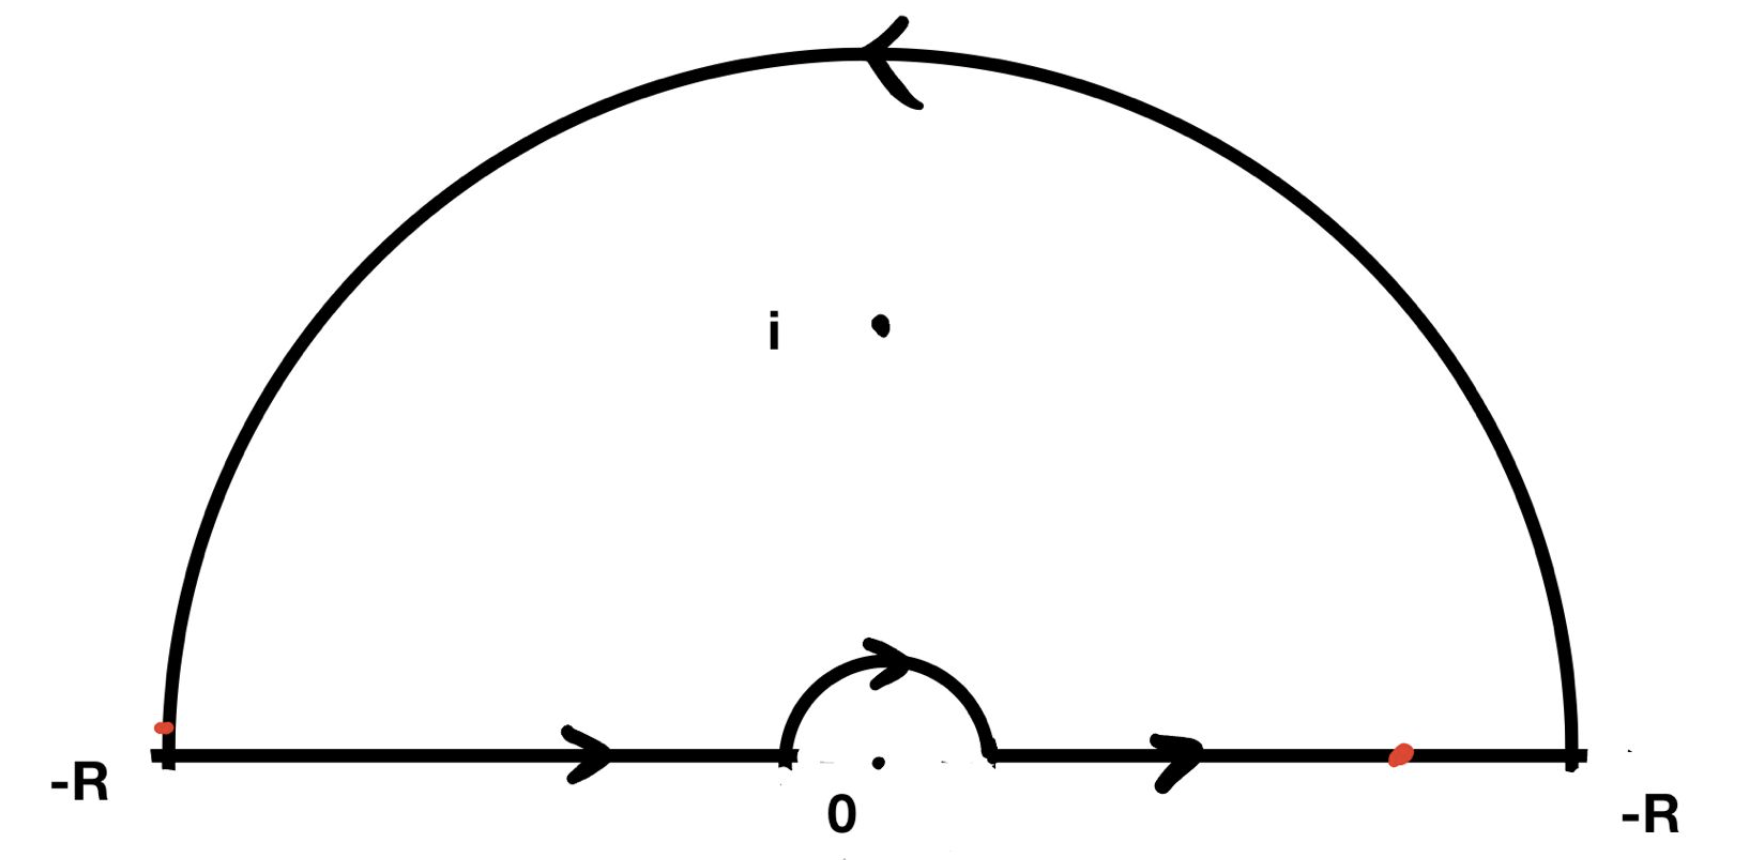
\includegraphics[width=0.76\linewidth]{figures/cycle.png}
%     \caption{半圆围道}
%     \label{banyuan}
% \end{figure}
\begin{center}
    \begin{tikzpicture}
        % 绘制坐标轴
        \draw[->] (-3.5, 0) -- (3.5, 0) node[right] {$\mathrm{Re}(z)$};
        \draw[->] (0, -1.5) -- (0, 3.5) node[above] {$\mathrm{Im}(z)$};
        % 绘制半圆形
        \draw[thick] (0,2) circle (0.3);
        \draw[thick,->] (3,0) arc (0:180:3);
          \draw[thick,<-] (0,1.7) arc (-90:90:0.3);
          \draw[thick,<-] (0.3,0) arc (0:180:0.3);
          \draw[thick,->](-3,0) -- (-0.3,0);
          \draw[thick,->](0.3,0) -- (3,0);
        % 绘制奇点标记
        \fill (0,0) circle (2pt) node[below right] {$0$};
        \fill (0,2) circle (2pt) node[above right] {$i$};
      \end{tikzpicture}
\end{center}
在半圆围道上,存在:
\begin{equation}\label{A1}
    \begin{aligned}
        & \lim _{R \rightarrow \infty} (\int_{0 }^{R }\frac{z^{-ik}}{z^2+1}\frac{dz}{z} +\int_{-R }^{0 }\frac{z^{-ik}}{z^2+1}\frac{dz}{z}) \\
    %    &=2\pi i(Res(f(t),i))=2\pi i \lim _{t \rightarrow i}\frac{t^{-ik}}{3t^2+1}\\
    %    &=-\pi ie^{\frac{k\pi}{2} } \\
       & =\lim _{R \rightarrow \infty} (\int_{0 }^{R }\frac{z^{-ik}}{z^2+1}\frac{dz}{z} -\int_{0 }^{-R }\frac{z^{-ik}}{z^2+1}\frac{dz}{z})\\
       & =\lim _{R \rightarrow \infty} (\int_{0 }^{R }\frac{z^{-ik}}{z^2+1}\frac{dz}{z} -\int_{0 }^{R }\frac{(ze^{i\pi})^{-ik}}{(ze^{i\pi})^2+1}\frac{d(-z)}{ze^{i\pi}})\\
       &=\lim _{R \rightarrow \infty} (\int_{0 }^{R }\frac{z^{-ik}}{z^2+1}\frac{dz}{z} -e^{k\pi }\int_{0 }^{R }\frac{z^{-ik}}{z^2+1}\frac{dz}{z}).
       \end{aligned}
\end{equation}
在该半圆形围道上使用留数定理:
\begin{equation}\label{A-9}
    \begin{aligned}
        &\int_{C} \frac{z^{-ik}}{z^2+1}\frac{dz}{z} =2 \pi i \cdot \operatorname{Res} f(z=i)+\pi i \cdot \operatorname{Res} f(z=0)\\
        &=2\pi i (\lim _{z \rightarrow i}\frac{z^{-ik}}{3z^2+1}+\lim _{z \rightarrow 0}\frac{z^{-ik}}{3z^2+1})=-\pi ie^{\frac{k\pi}{2} } + 0\\
        &=\lim _{R \rightarrow \infty} (\int_{0 }^{R }\frac{z^{-ik}}{z^2+1}\frac{dz}{z} +\int_{-R }^{0 }\frac{z^{-ik}}{z^2+1}\frac{dz}{z}) +\int_{\mathrm{arc}} \frac{z^{-ik}}{z^2+1}\frac{dz}{z}  
        \end{aligned}
\end{equation}
    其中,$\int_{\mathrm{arc}} \frac{z^{-ik}}{z^2+1}\frac{dz}{z}  $是半圆弧线上的积分,可以估算:
        \begin{equation}
            \left|\int_{\mathrm{arc}} \frac{z^{-ik}}{z^2+1}\frac{dz}{z}  \right| \leq \pi R \cdot \sup _{\text {arc }}\left|\frac{z^{-ik}}{z^3+z}\right| \leq \pi R \cdot \sup _{\operatorname{arc}} \frac{1}{\left|z^3+z\right|} \leq \frac{\pi R}{R^3+R-1}
            \end{equation}
    且:
    \begin{equation}\label{}
        \lim _{R \rightarrow \infty} \frac{\pi R}{R^3+R-1}=0
    \end{equation}
    所以:
    \begin{equation}\label{A2}
        \int_{\mathrm{arc}} \frac{z^{-ik}}{z^2+1}\frac{dz}{z} = 0
    \end{equation}
将式\ref{A1},\ref{A2}代入式\ref{A-9}可得:
\begin{equation}\label{}
    \begin{aligned}
    &\lim _{R \rightarrow \infty} \int_{0 }^{R }\frac{z^{-ik}}{z^2+1}\frac{dz}{z} = \frac{-\pi i e^{\frac{k\pi}{2}}}{1-e^{k\pi}}\\
    &= \frac{\pi i}{2\sinh\frac{k\pi}{2}}
\end{aligned}
\end{equation}
于是第二项积分为:
\begin{equation}\label{}
    \int_{-\infty }^{\infty } \frac{2e^{-ikx}}{e^{2x}+1} dx = \frac{\pi i}{\sinh\frac{k\pi}{2}}
\end{equation}
于是,双曲正切函数的傅立叶变换为:
\begin{equation}
    \begin{aligned}
      \int_{-\infty }^{\infty } \tanh (x)e^{-ikx}dx= -\frac{\pi i}{\sinh\frac{k\pi}{2}}
\end{aligned}
\end{equation}
